\begin{figure}[H]
\centering
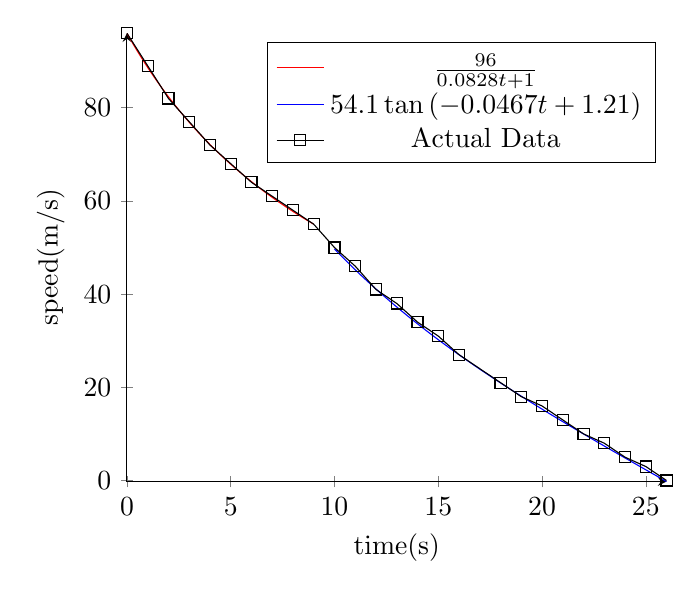
\begin{tikzpicture}
\begin{axis}[
    axis lines = left,
    xlabel = time(s),
    ylabel = speed(m/s),
]
%Below the red parabola is defined
\addplot [
    domain=0:9,
    samples=100, 
    color=red,
]
{96/(0.0828*x + 1)};
\addlegendentry{$\frac{96}{0.0828t + 1}$}
%Here the blue parabloa is defined
\addplot [
    domain=10:26, 
    samples=100, 
    color=blue,
    ]
    {54.1*tan((-0.0467*x + 1.21)*(180/3.1415))};
\addlegendentry{$54.1\tan{(-0.0467t+1.21)}$}

 \addplot[
    color=black,
    mark=square]
    coordinates {(0,96)(1,89)(2,82)(3,77)(4,72)(5,68)(6,64)(7,61)(8,58)(9,55)(10,50)(11,46)(12,41)(13,38)(14,34)(15,31)(16,27)(18,21)(19,18)(20,16)(21,13)(22,10)(23,8)(24,5)(25,3)(26,0)};
\addlegendentry{Actual Data}
\end{axis}
\end{tikzpicture}
\caption{Graph of model 3 for $m=115,000kg$}
\end{figure}

From this graph, we can clearly see that there is not much of a difference by taking $m=115000kg$. Just like with the other case, the difference is also very hard to see and taking $m=115,000kg$, doesn't have much of a difference on the model and the RMS error is also very low as it is 0.147. This means that not much has changed and that the model still very well models the landing of the aeroplane.